\thispagestyle{lichsutoanhocnone}
\pagestyle{lichsutoanhoc}
\graphicspath{{../lichsutoanhoc/pic/}}
\everymath{\color{lichsutoanhoc}}
\blfootnote{$^1$\color{lichsutoanhoc}Cộng tác viên Viện Toán học.}
\begingroup
\AddToShipoutPicture*{\put(0,616){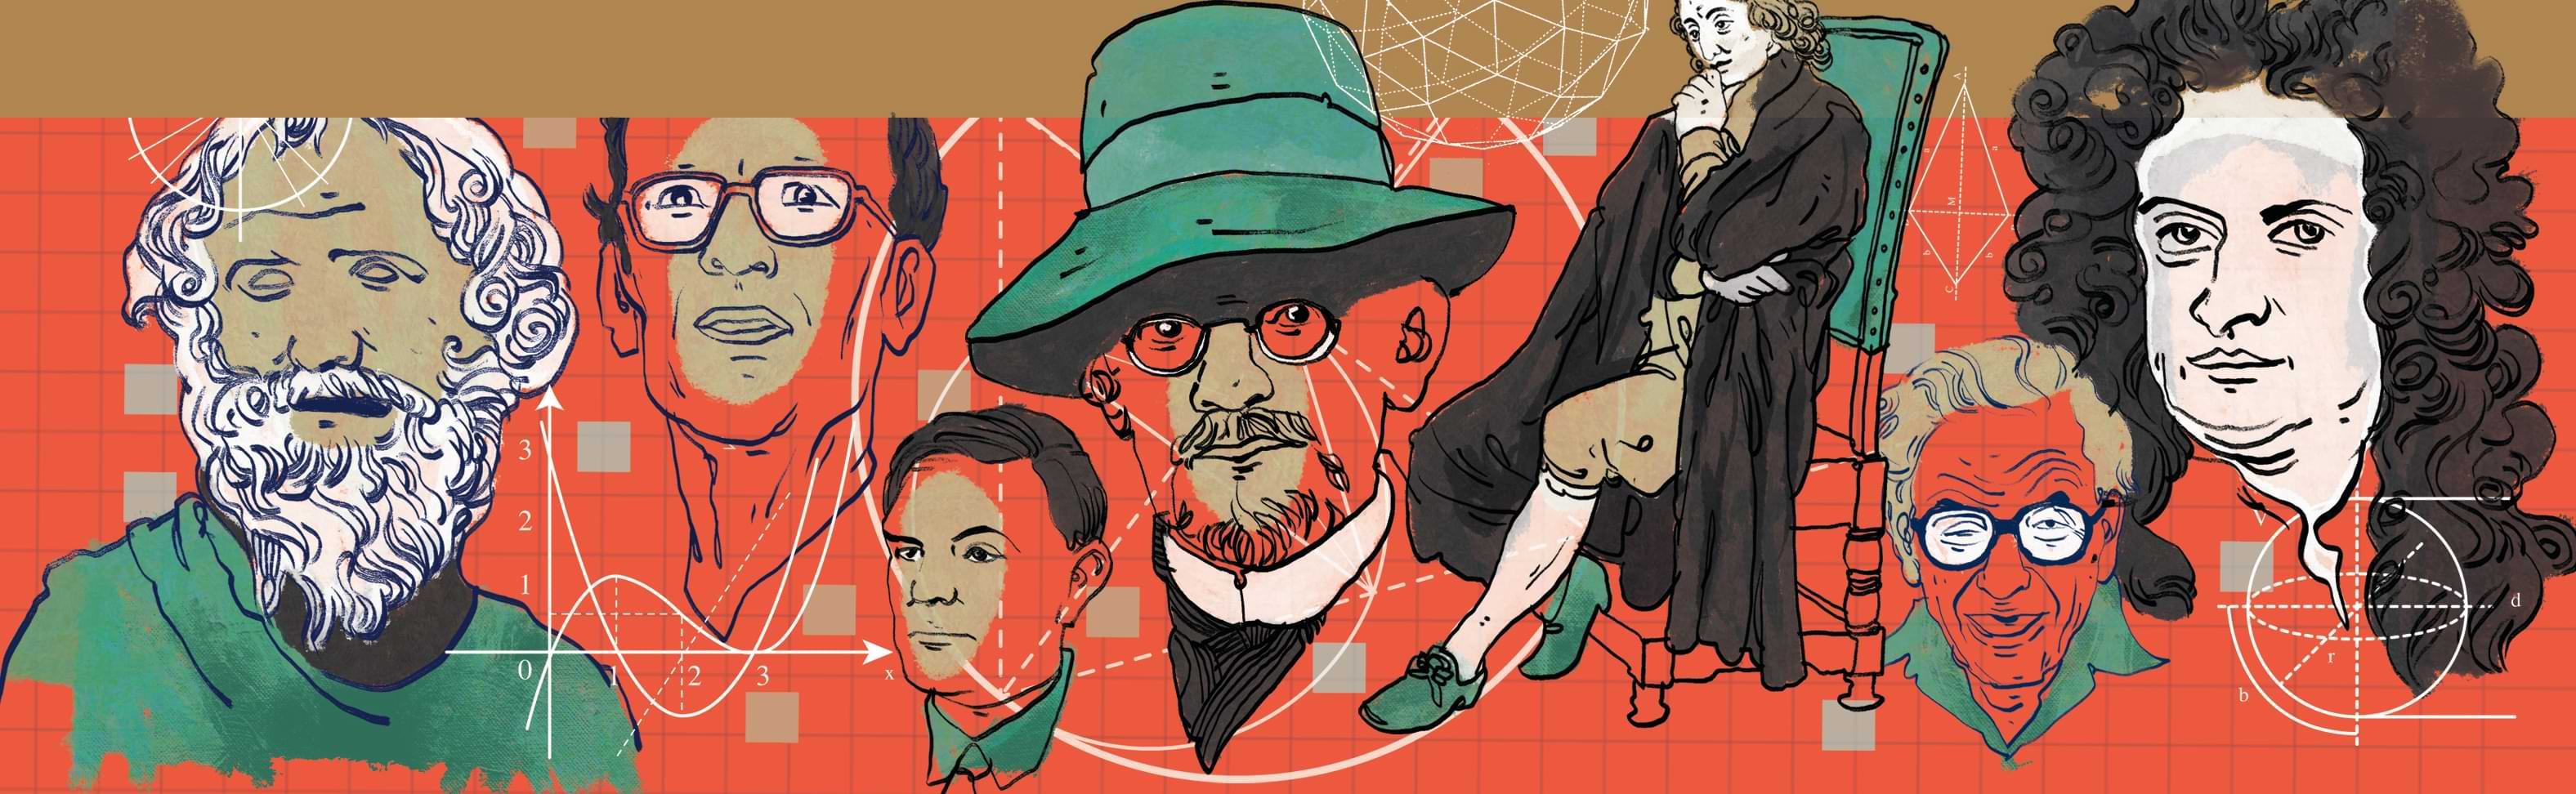
\includegraphics[width=19.3cm]{../bannerlichsu}}}
\AddToShipoutPicture*{\put(80,522){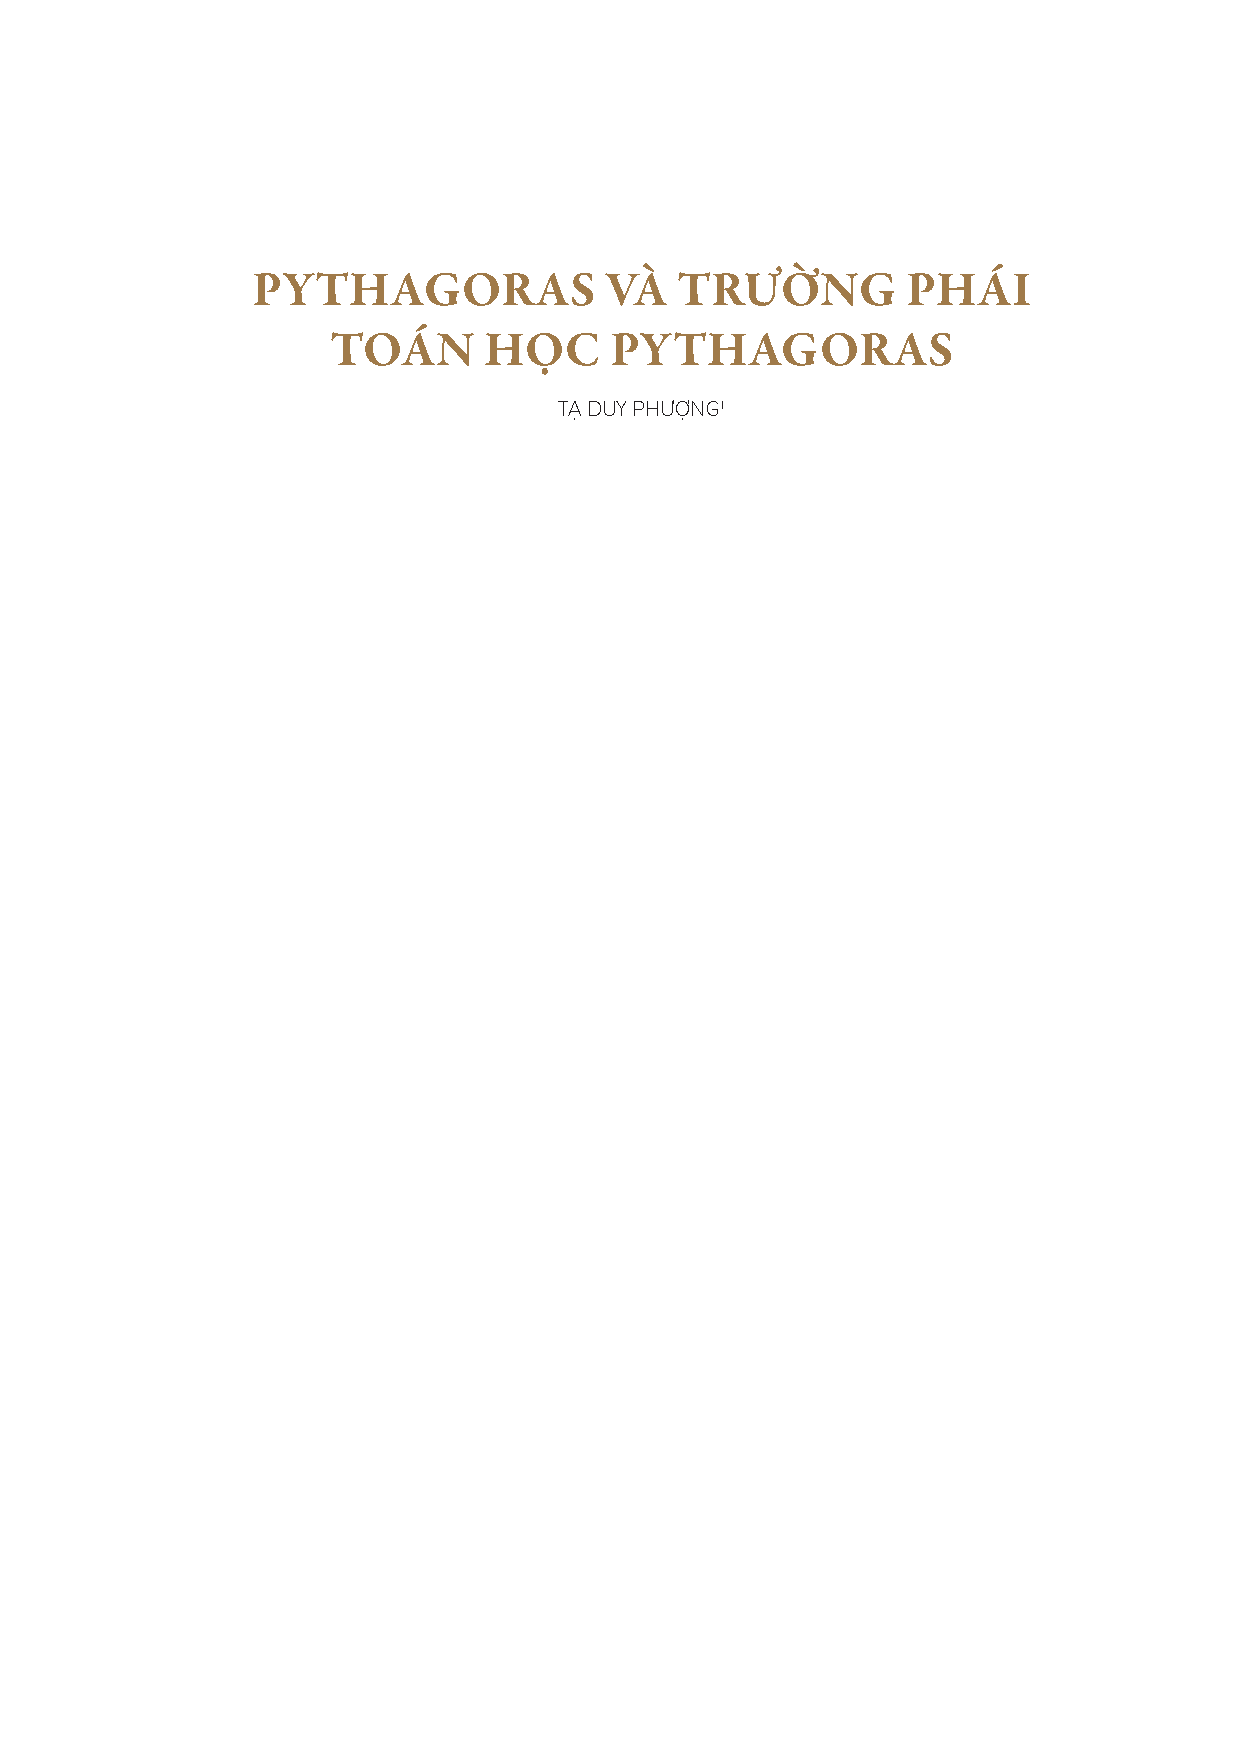
\includegraphics[scale=1]{../tieude.pdf}}}
\centering
\endgroup

\vspace*{180pt}

\begin{multicols}{2}
	\textbf{\color{lichsutoanhoc}Từ Thales đến Pythagoras}
	\vskip 0.05cm 
	Mặc dù Thales là người sáng lập trường phái triết học và toán học mang tên \textit{trường phái Ionia} hay \textit{trường phái Miletus} ở quê ông, chúng ta hoàn toàn mơ hồ về lịch sử hình học Hy Lạp trong giai đoạn chuyển tiếp từ Thales đến Pythagoras. Anaximander (khoảng $610-546$ trước CN) là nhà thiên văn học. Ông là người đầu tiên vẽ bản đồ Trái Đất có người ở, điều này liên quan đến việc tính các kích thước của Trái Đất. Do đó, rõ ràng Anaximander là một nhà toán học. Tuy nhiên, chưa biết ông có những đóng góp gì cho hình học. Sau Thales, Ameristus đã tham gia nghiên cứu và dường như cũng nổi tiếng trong hình học. Anaximander, Ameristus và Pythagoras là những học trò của Thales. Nhận thấy tài năng của Pythagoras, Thales đã truyền thụ cho chàng trai trẻ hết các kiến thức của mình\footnote[2]{\color{lichsutoanhoc}Burton, $[1]$, trang $90$.}.
	\vskip 0.05cm 
	Sau Thales và Ameristus, Pythagoras đã biến việc nghiên cứu hình học thành một nền giáo dục khai mở, kiểm tra các nguyên tắc của khoa học này ngay từ đầu và khám phá các định lý trong lĩnh vực toán học phi vật chất và trí tuệ\footnote[3]{\color{lichsutoanhoc}Thomas Heath, $[3]$, trang $139-140$.}.
	\begin{figure}[H]
		\vspace*{5pt}
		\centering
		\captionsetup{labelformat= empty, justification=centering}
		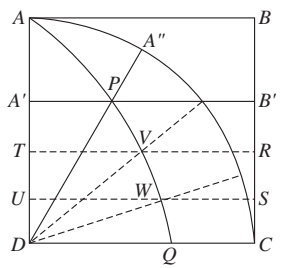
\includegraphics[width= 1\linewidth]{1}
		\caption{\small\textit{\color{lichsutoanhoc}Pythagoras: Bảo tàng Capitolino, Rome.}}
		\vspace*{-15pt}
	\end{figure}
	\textbf{\color{lichsutoanhoc}Tiểu sử Pythagoras} 
	\vskip 0.1cm
	Thông tin về Pythagoras khá mơ hồ. Ngay cả năm sinh của ông cũng có khá nhiều giả định: Pythagoras có thể sinh ra vào một trong các năm $590$, $586$, $584$, $582$, $572$, $569$ trước Công nguyên\footnote[4]{\color{lichsutoanhoc}Evans G. Valens, $[8]$, trang $23$.}  tại thị trấn Tigani trên đảo Samos của Hy Lạp và mất vào khoảng năm $497$ trước Công nguyên.
	\vskip 0.05cm
	Pythagoras đã đến thăm Ai Cập, Babylon và -- có thể -- thậm chí cả Ấn Độ. Trong thời gian du lịch, ông không chỉ tiếp thu toán học và thiên văn, mà còn cả các lý thuyết tôn giáo khác nhau. 
	\vskip 0.1cm
	Khoảng năm $545$ trước Công nguyên, ông thành lập một trường học ở Samos và sau khi Ba Tư chiếm đóng Samos, khoảng năm $530$ trước Công nguyên, ông định cư ở Crotone, miền Nam nước Ý, nơi ông cũng thành lập một trường học.
	\vskip 0.1cm
	Pythagoras là nhân vật nổi trội nhất trong thời kỳ chuyển tiếp giữa thời kỳ Cổ đại (Antiquity) và thời kỳ Cổ điển (Classical Period). Trong thế giới Cổ đại, các vị thần đóng vai trò trung tâm trong cuộc sống hàng ngày, có sự gắn bó chặt chẽ với thế giới vật chất, có sinh và diệt, sống và chết. Trong thế giới quan Cổ điển, các vị thần (hoặc thượng đế) được cho là có liên quan đến cá nhân, đạo đức với loài người. Thần thánh có thể được tìm thấy trong tâm hồn. Các hiện tượng tự nhiên được giải thích thông qua quan niệm về quan hệ nhân quả. Quan điểm hiện tại của chúng ta về thế giới dựa trên bản thân thế giới quan Cổ điển này là sản phẩm của triết học Pythagoras và các nhà tư tưởng tiền Socrates khác, và vẫn là nguồn gốc của nhiều phát triển hiện đại.\footnote[5]{\color{lichsutoanhoc}About Pythagoras, Pythagoras Foundation $[7]$}
	\begin{figure}[H]
		\vspace*{-5pt}
		\centering
		\captionsetup{labelformat= empty, justification=centering}
		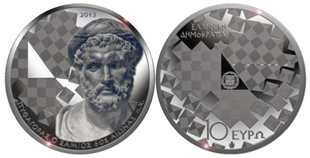
\includegraphics[width= 1\linewidth]{2}
		\caption{\small\textit{\color{lichsutoanhoc}Đồng bạc (Hy Lạp) $10$ Euro, $2013$. Đồng bạc tôn vinh nhà văn hóa Hy Lạp, Triết gia -- Pythagoras của Samos.}}
		\vspace*{-10pt}
	\end{figure}
	Pythagoras, tình cờ, gần như là người sinh cùng thời với Đức Phật, Khổng Tử và Lão Tử, ở vào thời điểm quan trọng trong sự phát triển triết học, tôn giáo và toán học trên thế giới.
	\vskip 0.1cm
	Khó có thể phủ nhận Pythagoras là một trong những nhân vật có ảnh hưởng nhất trong lịch sử. Đối với những người theo ông, dù bị lừa dối hay được truyền cảm hứng, niềm tin của họ đã được truyền bá khắp thế giới Hy Lạp. Sự hài hòa và những bí ẩn triết học và toán học là những phần thiết yếu của nghi lễ Pythagoras (Pythagorean rituals). Chưa bao giờ toán học lại đóng vai trò lớn như vậy trong cuộc sống và trong tôn giáo, như nó đã đóng trong cộng đồng Pythagoras. 
	\vskip 0.1cm
	Bản thân Pythagoras không để lại các bản viết. Hơn nữa, cộng đồng Pythagoras (Pythagorean societies) coi tài sản và kiến thức là của chung, các phát minh và khám phá không được ghi danh cho người cụ thể nào, vì vậy rất khó đoán định kết quả nào là của Pythagoras, kết quả nào là của học trò ông.  Có lẽ đặc điểm nổi bật nhất của hệ thống có trật tự mà Pythagoras xây dựng là nó duy trì sự tự tin khi theo đuổi các nghiên cứu triết học và toán học như một cơ sở đạo đức cho việc ứng xử cuộc sống.  Những từ ``Triết học" (``tình yêu của sự thông thái") và ``toán học" (``cái mà được học") được cho là do chính Pythagoras đặt ra để mô tả các hoạt động trí tuệ của ông.
	\vskip 0.1cm
	\textbf{\color{lichsutoanhoc}Những khám phá toán học được cho là của trường phái Pythagoras}
	\vskip 0.1cm
	Rõ ràng trường phái Pythagoras đã đóng một vai trò quan trọng trong toán học. Toán học Ả Rập và Lưỡng Hà (Mesopotamia) chủ yếu là áp dụng các quy tắc tính toán trong số học, đo đạc (ruộng đất) mà chưa đi đến các nguyên tắc chung.
	\vskip 0.1cm  
	Thales thường được coi là đã bắt đầu theo hướng đưa toán học lên thành một ngành khoa học, mặc dù đa số ủng hộ quan điểm của Eudemus và Proclus là điểm nhấn mới trong phát triển toán học là do trường phải Pythagoras tạo ra.
	\vskip 0.1cm
	Trong trường phái Pythagoras, toán học liên quan chặt chẽ đến trí tuệ hơn là các yêu cầu của cuộc sống thực tế.
	\vskip 0.1cm
	Các sách lịch sử toán học thường viết: \textit{kết quả này là của trường phái Pythagoras} (Pythagorean School)  hoặc của \textit{người} [thuộc trường phái] \textit{Pythagoras} (Pythagorean). Tuy nhiên, ý kiến chung thống nhất là Pythagoras chính là người đã nâng toán học thành một khoa học, và ông có những đóng góp đặc biệt trong số học và âm nhạc.
	\begin{figure}[H]
		\vspace*{-5pt}
		\centering
		\captionsetup{labelformat= empty, justification=centering}
		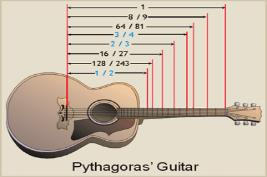
\includegraphics[width= 1\linewidth]{3}
%		\caption{\small\textit{\color{lichsutoanhoc}Đồng bạc (Hy Lạp) $10$ Euro, $2013$. Đồng bạc tôn vinh nhà văn hóa Hy Lạp, Triết gia -- Pythagoras của Samos.}}
		\vspace*{-15pt}
	\end{figure}
	Một học thuyết toán học quan trọng của trường phái Pythagoras là ``số lượng là bản chất của tất cả mọi thứ", rằng ``các con số, tức là các số nguyên dương, đã hình thành nguyên tắc tổ chức cơ bản của vũ trụ." Đối với trường phái Pythagoras, không chỉ tất cả các vật thể đã biết đều có số hoặc có thể được sắp xếp và đếm, mà những con số đó cũng là cơ sở của tất cả các hiện tượng. Ví dụ, một chòm sao trên trời có thể được đặc trưng bởi hai số: lượng các ngôi sao tạo nên nó và dạng hình học của nó, mà bản thân nó có thể được coi như được đại diện bởi một số. Chuyển động của các hành tinh có thể được biểu thị dưới dạng tỷ lệ của các con số. Hòa âm phụ thuộc vào tỷ lệ số: hai dây gảy với tỷ lệ độ dài $2:1$ cho một quãng tám, với tỷ lệ $3:2$ cho một phần năm và với tỷ lệ $4:3$ cho tỷ lệ một phần tư. Trong số những khoảng này, toàn bộ thang âm nhạc có thể được tạo ra. Và cuối cùng, tam giác có các cạnh theo tỷ lệ $3:4:5$ thiết lập một quan hệ giữa cạnh và góc. Với sự quan tâm của Pythagoras đối với số như một nguyên tắc cơ bản của vũ trụ, điều tự nhiên là trường phái Pythagoras đã nghiên cứu tỷ mỉ các tính chất của các số nguyên dương, mà ngày nay ta gọi là các yếu tố của lý \linebreak thuyết số.
	\begin{figure}[H]
		\vspace*{-5pt}
		\centering
		\captionsetup{labelformat= empty, justification=centering}
		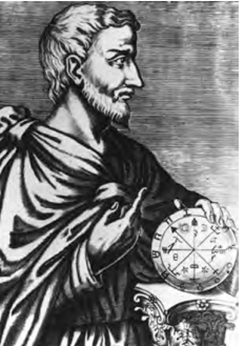
\includegraphics[width= 0.7\linewidth]{4}
		\caption{\small\textit{\color{lichsutoanhoc}Pythagoras (The Bettmann Archive).}}
		\vspace*{-10pt}
	\end{figure}
	\textbf{\color{lichsutoanhoc}Số và hình của trường phái Pythagoras}
	\vskip 0.05cm
	Cuốn sách \textit{Introductio Arithmeticae} (Nhập môn số học [$6$]) của Nicomachus xứ Geraca ($60-120$), người thuộc trường phái Pythagoras, khá nổi tiếng và phổ biến cho tới tận năm 1500, đã trình bày phần lớn các kết quả của Pythagoras và các học trò về số và hình.  
	\vskip 0.05cm
	Các số của trường phái Pythagoras thường được biểu diễn thông qua các hình: số tam giác, số vuông, số đa giác.
	\vskip 0.1cm
	Các số $t_1 =1, t_2 = 3, t_3 = 6, t_4 = 10$ là các số tam giác (triangular number), vì chúng có thể xếp như tam giác đều:  
	\begin{figure}[H]
		\vspace*{-5pt}
		\centering
		\captionsetup{labelformat= empty, justification=centering}
		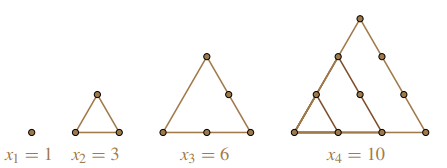
\includegraphics[width= 1\linewidth]{5}
%		\caption{\small\textit{\color{lichsutoanhoc}Pythagoras (The Bettmann Archive).}}
		\vspace*{-10pt}
	\end{figure}
	Tương tự, các số $s_1 = 1$, $s_2 = 4$, $s_3 = 9$, $s_4 = 16$ là các số vuông (số bình phương, square number), vì chúng có thể biểu diễn dưới dạng hình vuông:
	\begin{figure}[H]
%		\vspace*{5pt}
		\centering
		\captionsetup{labelformat= empty, justification=centering}
		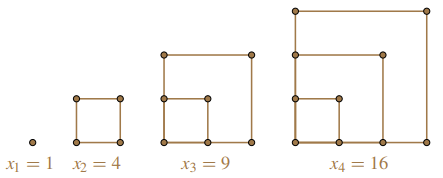
\includegraphics[width= 1\linewidth]{6}
		%		\caption{\small\textit{\color{lichsutoanhoc}Pythagoras (The Bettmann Archive).}}
		\vspace*{-25pt}
	\end{figure}
	Có thể tìm ra một số quy luật về số nhờ cách biểu diễn qua hình vẽ trên. Thí dụ, quan hệ giữa các số tam giác và số vuông như sau:
	\setlength{\abovedisplayskip}{4pt}
	\setlength{\belowdisplayskip}{4pt}
	\begin{align*}
		s_2 = t_1 + t_2, s_3 = t_2 + t_3, s_4 = t_3 + t_4,
	\end{align*}
	\begin{figure}[H]
		\vspace*{-15pt}
		\centering
		\captionsetup{labelformat= empty, justification=centering}
		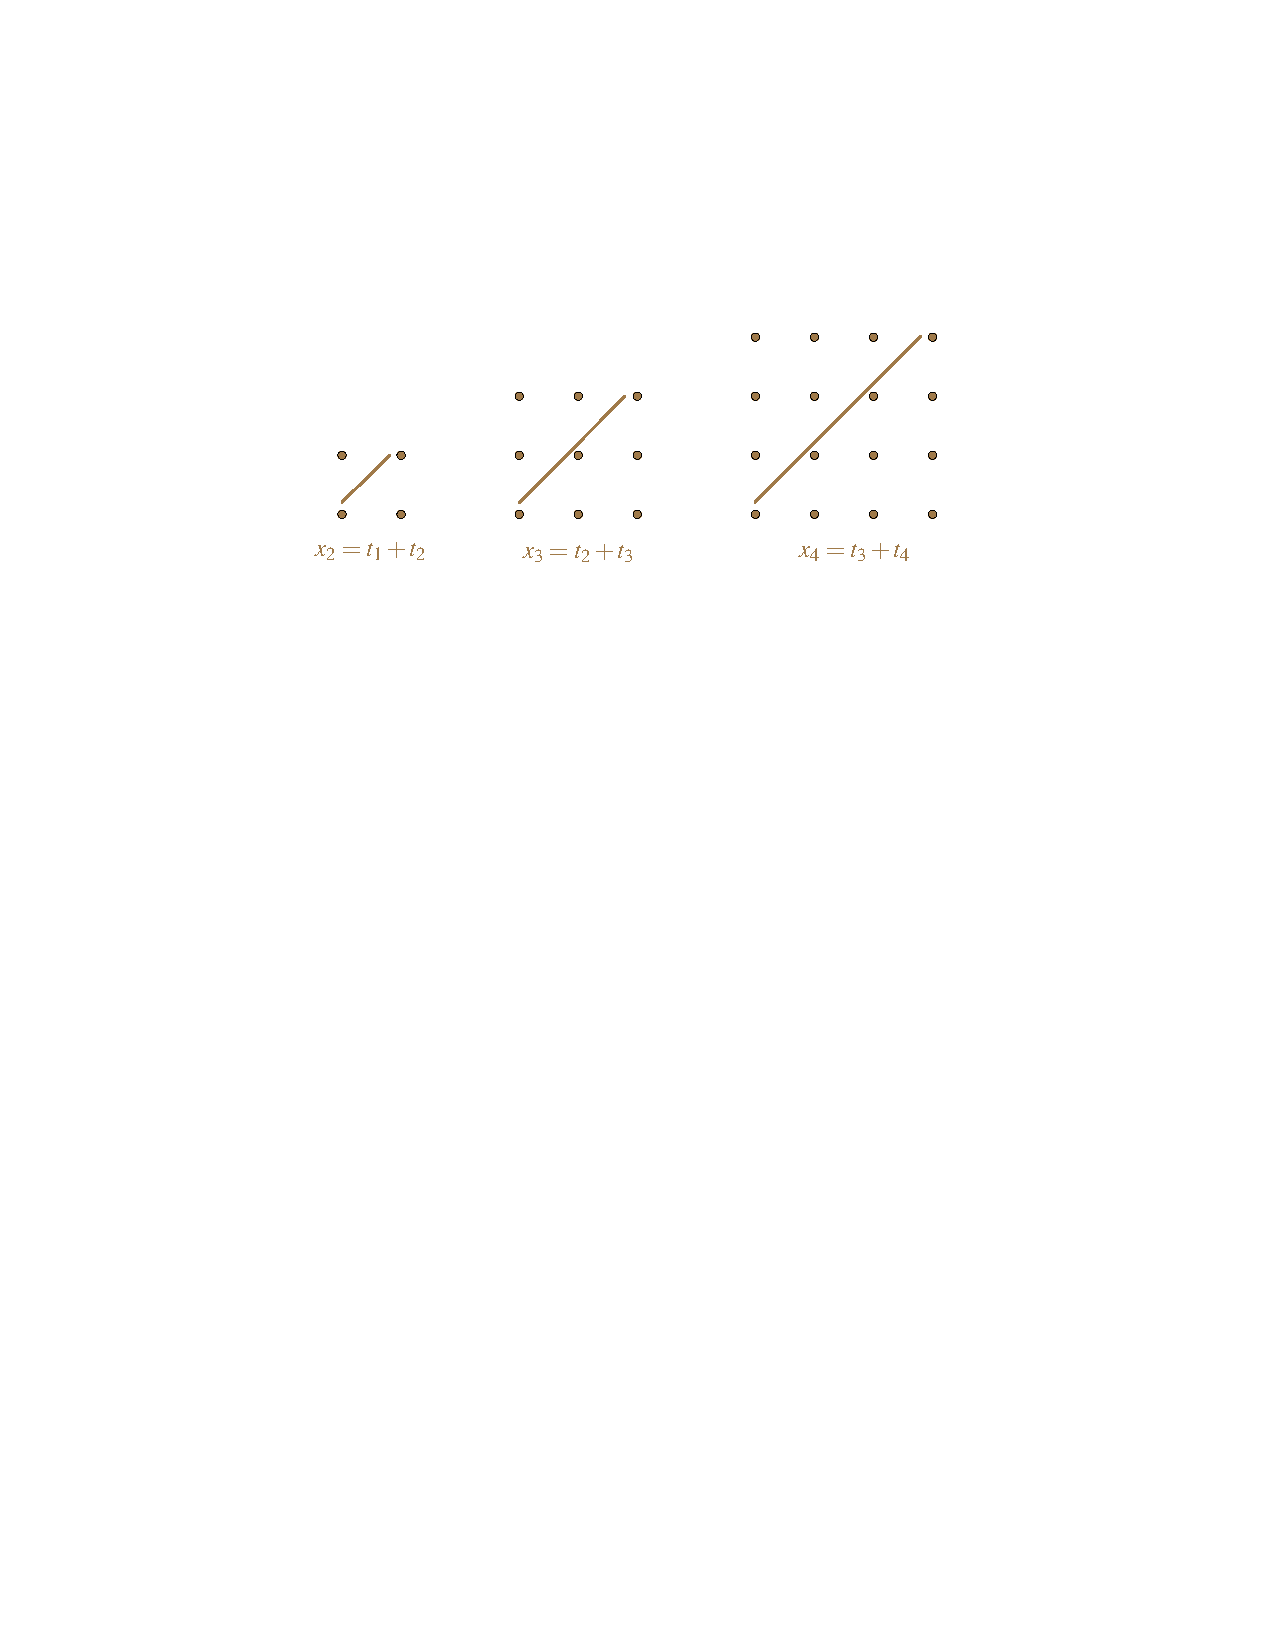
\includegraphics[width= 1\linewidth]{7.pdf}
		\vspace*{-25pt}
	\end{figure}
	\begin{align*}
			{t_n} &= {t_{n - 1}} + n = \left( {{t_{n - 2}} + \left( {n - 1} \right)} \right) + n = ...\\
			&= {t_1} + 2 + 3 + ... + \left( {n - 1} \right) + n\\
			&= 1 + 2 + ... + \left( {n - 1} \right) + n.
	\end{align*}
	Xếp hai số tam giác, mỗi số tam giác biểu diễn $t_n$ (tức là mỗi tam giác số chứa $n$  dòng, có $1,2,\ldots,\left( {n - 1} \right),n$ dấu chấm) thành một hình chữ nhật $n \times (n+1)$ thí  dụ, $t_5$,  như hình dưới:
	\begin{figure}[H]
		\vspace*{-5pt}
		\centering
		\captionsetup{labelformat= empty, justification=centering}
		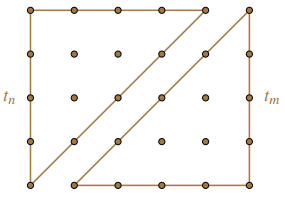
\includegraphics[width= 0.65\linewidth]{8}
		%		\caption{\small\textit{\color{lichsutoanhoc}Pythagoras (The Bettmann Archive).}}
		\vspace*{-10pt}
	\end{figure}
	Như vậy, ta có  $n \times \left( {n + 1} \right)$ dấu chấm, và do~đó
	\begin{align*}
		2{t_n} = n \times \left( {n + 1} \right) \text{ hay } {t_n} = \frac{{n\left( {n + 1} \right)}}{2}.
	\end{align*}  
	Vậy tổng của $n$ số tự nhiên đầu tiên bằng
	\begin{align*}
		1 \!+\! 2 \!+\!\ldots\! +\! \left(\! n \!-\! 1 \!\right) \!+\! n \!=\! {t_n} \!=\! \frac{{n\left(\! {n \!+\! 1} \right)}}{2}. \tag{$1$}
	\end{align*}
	Với công thức ($1$), có thể coi số vuông thứ $n$  chính là tổng của hai số tam giác liên tiếp:
	\begin{align*}
		{s_n} = {n^2} = \frac{{n(n + 1)}}{2} + \frac{{\left( {n - 1} \right)n}}{2} = {t_n} + {t_{n - 1}}.
	\end{align*}
	Tương tự, tổng của $n$  số lẻ đầu tiên có thể tìm được như sau. Quan sát thấy một hình vuông gồm  $n$  chấm trên một cạnh có thể được chia thành một hình vuông nhỏ hơn cạnh $n-1$   và một đường viền hình chữ L (Hình dưới, bên trái). 
	\begin{figure}[H]
		\vspace*{-5pt}
		\centering
		\captionsetup{labelformat= empty, justification=centering}
		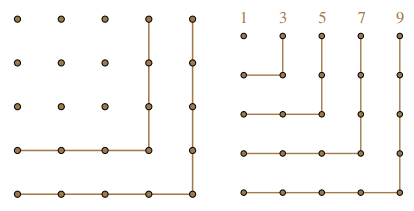
\includegraphics[width=0.85\linewidth]{9a}
		%		\caption{\small\textit{\color{lichsutoanhoc}Pythagoras (The Bettmann Archive).}}
		\vspace*{-15pt}
	\end{figure}
	Bằng cách lặp lại phép chia nhỏ này, như trong sơ đồ bên phải, rõ ràng là sự khác biệt giữa các ô vuông lồng nhau liên tiếp tạo ra chuỗi các số lẻ; do đó
	\begin{align*}
		1 + 3 + 5 + ... + \left( {2n - 3} \right) + \left( {2n - 1} \right) = {n^2}.
	\end{align*}
	Trường phái Pythagoras có thể đã chứng minh kết quả này bằng cách xét $n$ đẳng thức
	\begin{align*}
		&1^2 = 1;\\[-0.5ex]
		&2^2 - 1^2 = 3;\\[-0.5ex]
		&{3^2} - {2^2} = 5;\\[-0.5ex]
		&{4^2} - {3^2} = 7;\\[-0.5ex]
		&\ldots\\[-0.5ex]
		&{n^2} - {\left( {n - 1} \right)^2} = 2n - 1.
	\end{align*}
	Cộng vế với vế các đẳng thức này, ta được
	\begin{align*}
		{n^2} = 1 + 3 + 5 + ... + \left( {2n - 3} \right) + \left( {2n - 1} \right).
	\end{align*}
	\textbf{\color{lichsutoanhoc}Lý thuyết số tượng hình} (The Theory of Figurative Numbers)
	\vskip 0.1cm
	Những người theo trường phái Pythagoras không thể ngờ rằng lý thuyết về các con số lại thu hút sự chú ý của các học giả sau này. Năm $1654$, nhà toán học--triết học Pascal $(1623-1662)$ đã viết \textit{Chuyên luận về các số tam giác} (\textit{Traité du triangle arithmétique}), trong đó ông khẳng định rằng mọi số nguyên dương là tổng của ba (hoặc ít hơn) số tam giác. Ví dụ,
	\begin{align*}
			&16 = 6 + 10;\quad 25 = 1 + 3 + 21;\\
			&39 = 3 + 15 + 21;\quad 150 = 6 + 66 + 78; \ldots
	\end{align*}
	Kết quả đáng chú ý này đã được phỏng đoán bởi Fermat $(1607-1665)$ trong một bức thư gửi Mersenne  $(1588-1648)$ vào năm $1636$ và lần đầu tiên được chứng minh bởi Gauss $(1777-1855)$  vào năm $1801$.
	\vskip 0.1cm
	Một mô hình thú vị khác có thể được quan sát từ các phương trình sau:
	\begin{align*}
			&1 = {1^3} = t_1^2;\\[-0.5ex]
			&{1^3} + {2^3} = 9 = t_2^2;\\[-0.5ex]
			&{1^3} + {2^3} + {3^3} = 36 = t_3^2; \\[-0.5ex]
			&{1^3} + {2^3} + {3^3} + {4^3} = 100 = t_4^2;\ldots
	\end{align*}
	Vậy
	\begin{align*}
		{1^3} + {2^3} + {3^3} + {4^3} + ... + {n^3} = t_n^2.
	\end{align*}
	Nhận xét bất ngờ này, liên hệ tổng các số lập phương với các số tam giác, thường được cho là của Nicomachus (thế kỷ I).
	\vskip 0.1cm
	Tìm công thức tính tổng bình phương của $n$  số tự nhiên đầu tiên mất nhiều thời gian và cố gắng hơn. 
	\vskip 0.1cm
	Đầu tiên chúng ta xét trường hợp $n=4$ từ đó tổng quát hóa cho trường hợp $n$  bất kỳ. 
	\vskip 0.1cm
	Đặt các hình vuông có chứa  dấu chấm liền kề nhau như hình dưới.
	\begin{figure}[H]
		\vspace*{-5pt}
		\centering
		\captionsetup{labelformat= empty, justification=centering}
		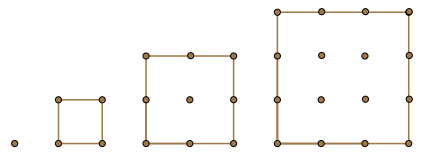
\includegraphics[width= 1\linewidth]{10}
		%		\caption{\small\textit{\color{lichsutoanhoc}Pythagoras (The Bettmann Archive).}}
		\vspace*{-15pt}
	\end{figure}
	Tiếp theo ta thêm vào các dòng $1$, $3$, $6$, $10$ chấm để được hình chữ nhật với chiều dài là $1+2+3+4$ và chiều cao là $4+1$ (hình dưới).  
	\begin{figure}[H]
		\vspace*{-5pt}
		\centering
		\captionsetup{labelformat= empty, justification=centering}
		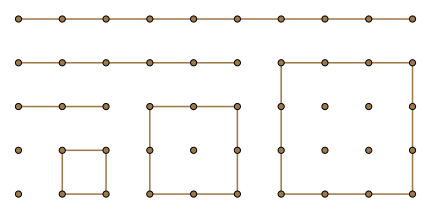
\includegraphics[width= 1\linewidth]{11}
		%		\caption{\small\textit{\color{lichsutoanhoc}Pythagoras (The Bettmann Archive).}}
		\vspace*{-5pt}
	\end{figure}
	Tính số các chấm trên các dòng và các hình vuông, ta được
	\begin{align*}
			&\left( {{1^2} + {2^2} + {3^2} + {4^2}} \right) + \left( {1 + 3 + 6 + 10} \right)\\
			= \,&\left( {1 + 2 + 3 + 4} \right)\left( {4 + 1} \right).
	\end{align*}
	Hay
	\begin{align*}
		\left( {{1^2} + {2^2} + {3^2} + {4^2}} \right) &= 10 \cdot 5 - 20 = 30 \\
		&= \frac{{4 \cdot 5 \cdot 9}}{6}.
	\end{align*}
	Tương tự, với $n=5$   ta có:
	\begin{figure}[H]
		\vspace*{-10pt}
		\centering
		\captionsetup{labelformat= empty, justification=centering}
		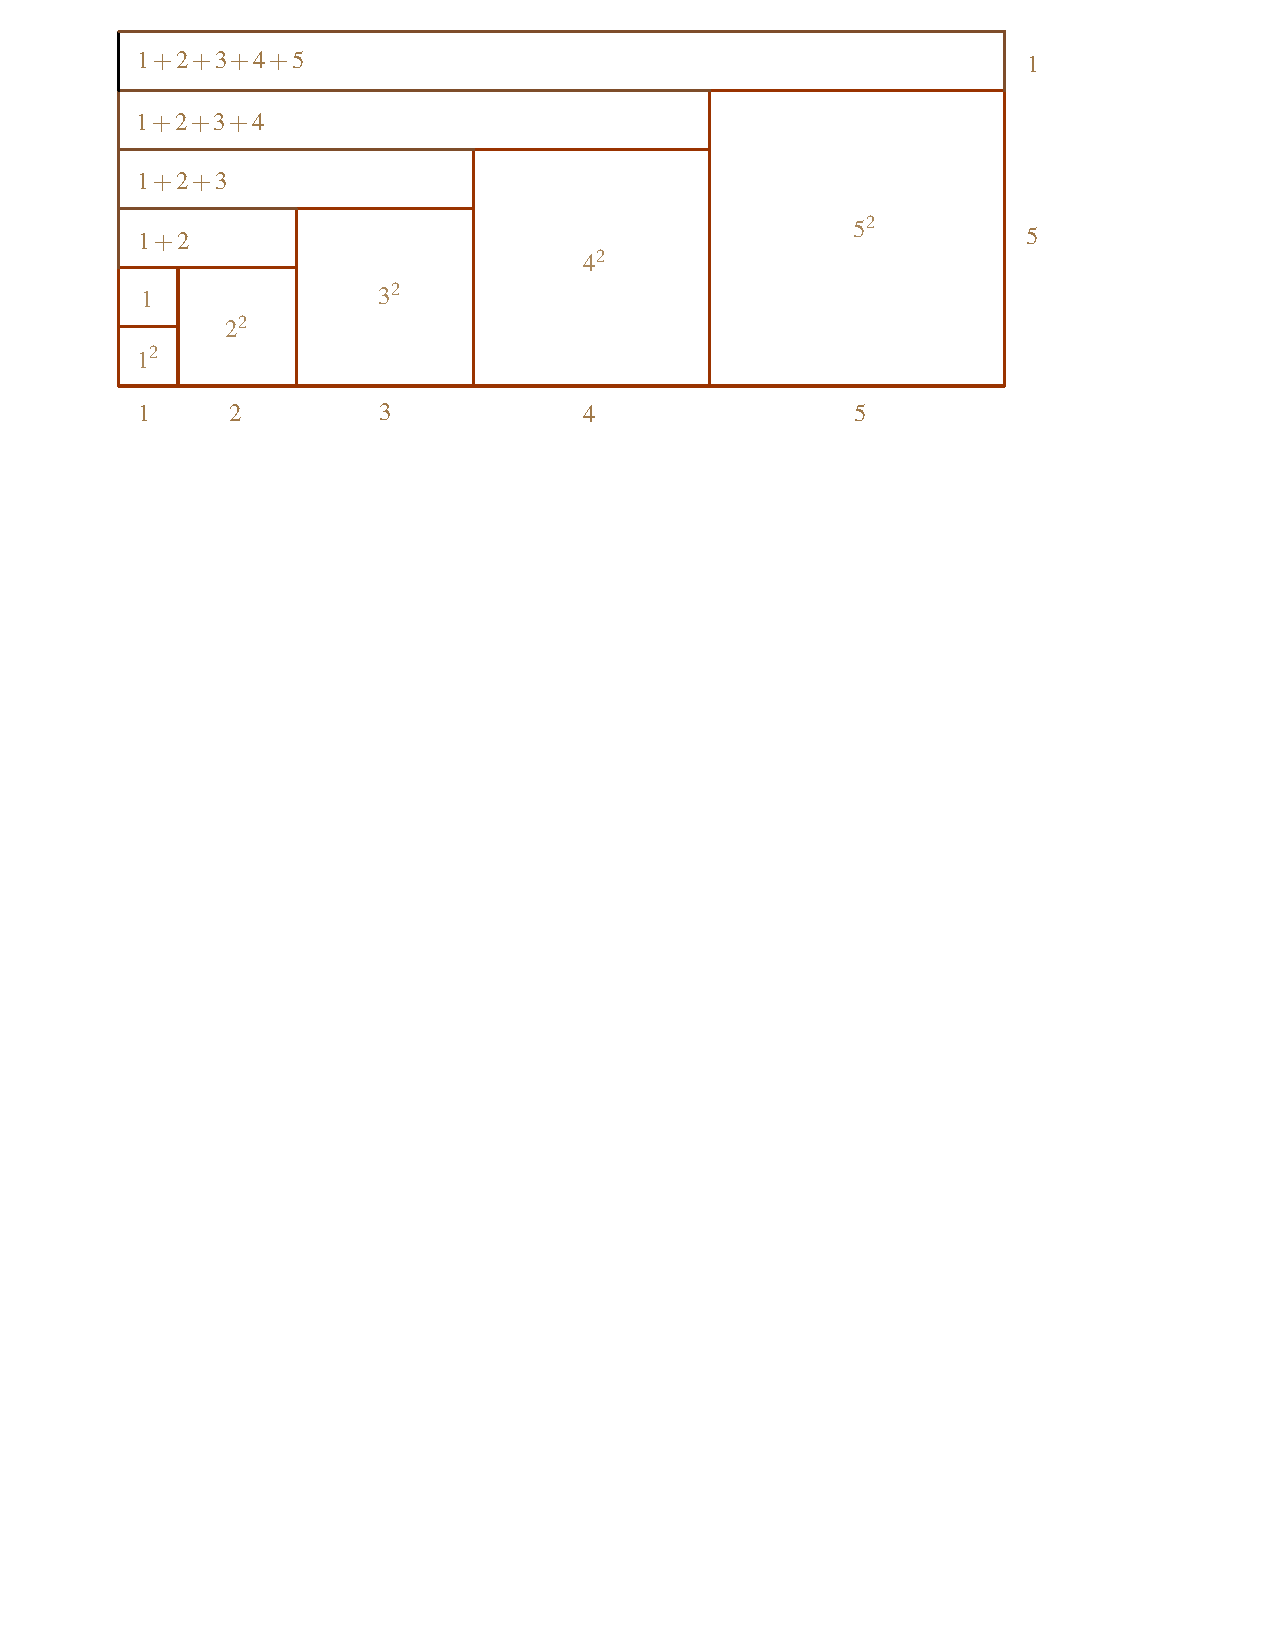
\includegraphics[width= 1\linewidth]{12.pdf}
		%		\caption{\small\textit{\color{lichsutoanhoc}Pythagoras (The Bettmann Archive).}}
		\vspace*{-20pt}
	\end{figure}
	Tổng quát, ta có thể tìm được tổng 
	\begin{align*}
		S: = {1^2} + {2^2} + {3^2} + ... + {n^2}
	\end{align*}
	như sau. Thêm 
	\begin{align*}
		&1 + \left( {1 + 2} \right) + \left( {1 + 2 + 3} \right) +  \ldots  \\[-0.5ex]
		&+ \left( {1 + 2 + 3 +  \ldots  + n} \right)
	\end{align*}
	dấu chấm vào các dòng của các hình vuông, ta được
	\begin{align*}
			&\left( {{1^2} + {2^2} + {3^2} + ... + {n^2}} \right)+ \left[ 1 + \left( {1 + 2} \right)\right.\\[-0.6ex]
			&\left. + \left( {1 + 2 + 3} \right) +  \ldots  + \left( {1 + 2 + 3 +  \ldots  + n} \right) \right]
	\end{align*}
	dấu chấm. Mặt khác, số dấu chấm trong hình chữ nhật bằng   $\left( {1 + 2 + 3 + ... + n} \right)\left( {n + 1} \right)$.
	\vskip 0.1cm 
	Như vậy, 
	\begin{align*}
			&\left( {{1^2} + {2^2} + {3^2} + ... + {n^2}} \right)+ \left[1 + \left( {1 + 2} \right) \right.\\[-0.6ex]
			&\left.+ \!\left( {1 \!+\! 2 \!+\! 3} \right) \!+\!  \ldots \! +\! \left( {1 \!+\! 2 \!+\! 3 \!+\!  \ldots  \!+\! n} \right) \right]\\[-0.6ex]
			=&\left( {1 + 2 + 3 + ... + n} \right)\left( {n + 1} \right).
	\end{align*}
	Biểu thức trên có thể viết dưới dạng
	\begin{align*}
		&S \!+\! \left(\!\frac{{1 \!\cdot\! 2}}{2} + \frac{{2 \!\cdot\! 3}}{2} + \frac{{3 \!\cdot\! 4}}{2} + ... + \frac{{n\left( {n + 1} \right)}}{2} \!\right) \\[-1ex]
		&= \frac{{n{{\left( {n + 1} \right)}^2}}}{2}.\\[-1ex]
		\Leftrightarrow\, &S + \frac{1}{2}\left( 1 \cdot \left( {1 + 1} \right) + 2\left( {2 + 1} \right) + 3\left( {3 + 1} \right)\right. \\[-1ex]
		&\left.+ ... + n\left( {n + 1} \right) \right)= \frac{{n{{\left( {n + 1} \right)}^2}}}{2}.
	\end{align*}
	\begin{align*}
		\Leftrightarrow \,&S + \frac{1}{2}\left( \left( {{1^2} + {2^2} + ... + {n^2}} \right)\right. \\
		&\left.+ \left( {1 + 2 + ... + n} \right) \right) = \frac{{n{{\left( {n + 1} \right)}^2}}}{2}.\\
		\Leftrightarrow \,&S + \frac{S}{2} + \frac{{n\left( {n + 1} \right)}}{4} = \frac{{n{{\left( {n + 1} \right)}^2}}}{2}\\
		\Leftrightarrow \,&\frac{{3S}}{2} = \frac{{n{{\left( {n + 1} \right)}^2}}}{2} - \frac{{n\left( {n + 1} \right)}}{4} \\
		&= \frac{{n\left( {n + 1} \right)\left( {2n + 1} \right)}}{4}.
	\end{align*}
	Vậy 
	\begin{align*}
		S &= {1^2} + {2^2} + ... + {n^2} \\
		&= \frac{{n\left( {n + 1} \right)\left( {2n + 1} \right)}}{6}. \tag{$2$}
	\end{align*}
	Fibonacci đã sử dụng đẳng thức
	\begin{align*}
		&k(k + 1)(2k + 1) \\
		= &(k - 1)k(2k - 1) + 6{k^2} \tag{$*$}
	\end{align*}
	để đi đến đẳng thức trên như sau.
	
	Thay $k = 1,2,...,n$  trong đẳng thức trên, ta được
	\begin{align*}
		&1 \cdot 2 \cdot 3 = 6 \cdot {1^2};\\
		&2 \cdot 3 \cdot 5 = 1 \cdot 2 \cdot 3 + 6 \cdot {2^2};\\
		&3 \cdot 4 \cdot 7 = 2 \cdot 3 \cdot 5 + 6 \cdot {3^2};\\
		&...\\
		&\left( {n - 1} \right)n\left( {2n - 1} \right) = \left( {n - 2} \right)\left( {n - 1} \right)\left( {2n - 3} \right)\\
		&+ 6{\left( {n - 1} \right)^2};\\
		&n\left( {n + 1} \right)\left( {2n + 1} \right) = \left( {n - 1} \right)n\left( {2n - 1} \right) + 6{n^2}.
	\end{align*}
	Cộng vế với vế các đẳng thức này ta đi đến
	\begin{align*}
		n\left( {n + 1} \right)\left( {2n + 1} \right) = 6\left( {{1^2} + {2^2} + ... + {n^2}} \right)
	\end{align*}
	hay
	\begin{align*}
		{1^2} + {2^2} + {3^2} + ... + {n^2} = \frac{{n\left( {n + 1} \right)\left( {2n + 1} \right)}}{6}.
	\end{align*}
	\textbf{\color{lichsutoanhoc}Định lý Pythagoras}
	\vskip 0.1cm
	\textit{Tam giác $ABC$ với ba cạnh $a,b,c$  là tam giác vuông tại $C$  khi và chỉ khi $c^2 =a^2 + b^2$}.
	\vskip 0.1cm
	\textit{\color{lichsutoanhoc}Chứng minh.} Hình vuông cạnh $a+b$  được chia thành hai hình vuông nhỏ hơn cạnh $a$  và $b$  tương ứng, và hai hình chữ nhật bằng nhau có cạnh $a$  và $b$.  Mỗi hình chữ nhật này lại chia thành hai tam giác vuông bằng nhau bằng cách kẻ đường chéo $c$ (Hình $1$, trái). Bốn hình tam giác có thể được sắp xếp trong một hình vuông khác cạnh $a+b$ (Hình $1$, phải).  
	\begin{figure}[H]
		\vspace*{-5pt}
		\centering
		\captionsetup{labelformat= empty, justification=centering}
		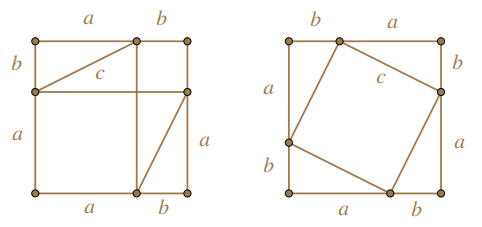
\includegraphics[width= 1\linewidth]{13}
		\caption{\small\textit{\color{lichsutoanhoc}Hình $1$. Chứng minh của định lý Pythagoras.}}
		\vspace*{-10pt}
	\end{figure}
	Diện tích của cùng một hình vuông cạnh $a+b$  có thể biểu diễn bằng hai cách: 
	\vskip 0.1cm
	Diện tích hình vuông cạnh  $a+b$ bằng tổng diện tích của hai hình vuông cạnh $a$ và cạnh $b$  với tổng diện tích hai hình chữ nhật (Hình $1$, trái):
	\begin{align*}
		{\left( {a + b} \right)^2} = {a^2} + {b^2} + 2ab.
	\end{align*}
	Mặt khác, diện tích hình vuông cạnh $a+b$  bằng tổng diện tích hình vuông cạnh $c$  và bốn lần diện tích tam giác vuông có các cạnh góc vuông $a$ và $b$  (Hình $1$, phải):
	\begin{align*}
		{\left( {a + b} \right)^2} = {c^2} + 4\left( {\frac{{ab}}{2}} \right).
	\end{align*}
	Suy ra $c^2 = a^2 + b^2$.
	\vskip 0.1cm 
	Những chứng minh bằng kỹ thuật cắt ghép hình đơn giản như trên có thể đã được làm trong một số nền văn minh khác. Tuy nhiên, không có một cơ sở nào để nói rằng người Ai Cập đã biết định lý Pythagoras.
	\vskip 0.1cm
	Có thể tìm thấy chứng minh Định lý Pythgoras trong cuốn sách \textit{Chu bễ toán kinh} (周髀算经) trong nền văn minh Trung Hoa. Thật là khó để xác định được chính xác thời gian xuất hiện của cuốn sách này. Tuy nhiên, có thể khẳng định phần cổ nhất của nó có niên đại trước năm $600$ trước Công nguyên. Chứng minh Định lý Pythagoras nhờ Hình $2$ có trong cuốn \textit{Cửu chương toán thuật} (九章算術) do Lưu Huy (Liu Hui) viết năm $263$. 
	\begin{figure}[H]
		\vspace*{5pt}
		\centering
		\captionsetup{labelformat= empty, justification=centering}
		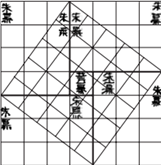
\includegraphics[width= 0.5\linewidth]{14}
		\caption{\small\textit{\color{lichsutoanhoc}Hình $2$. Định lý Pythagoras trong Cửu chương toán thuật.}}
		\vspace*{-10pt}
	\end{figure}
	Văn minh Trung Hoa được phát triển hoàn toàn độc lập với văn minh Babilon và văn minh Ai Cập. 
	\vskip 0.1cm
	Chứng minh bằng cách ghép hình gây cảm hứng và sự ngưỡng mộ vì sự đơn giản đến sang trọng của nó. Nhà toán học người Hindu Bhaskara ($1114-1185$) đã vẽ hai hình dưới đây trong \textit{Vijaganita} (Tính toán gốc): bốn tam giác vuông đặt trong hình vuông có cạnh là cạnh huyền $c$, ở giữa vẫn còn một hình vuông có cạnh $a-b$ (Hình $3$, trái). Hình vuông này và bốn hình tam giác sau đó được xếp lại để tạo nên diện tích của hai hình vuông cạnh $a$ và $b$  (Hình $3$, phải). Và ông chỉ viết một chữ: ``Behold -- Nhìn này!"
	\begin{figure}[H]
		\vspace*{-5pt}
		\centering
		\captionsetup{labelformat= empty, justification=centering}
		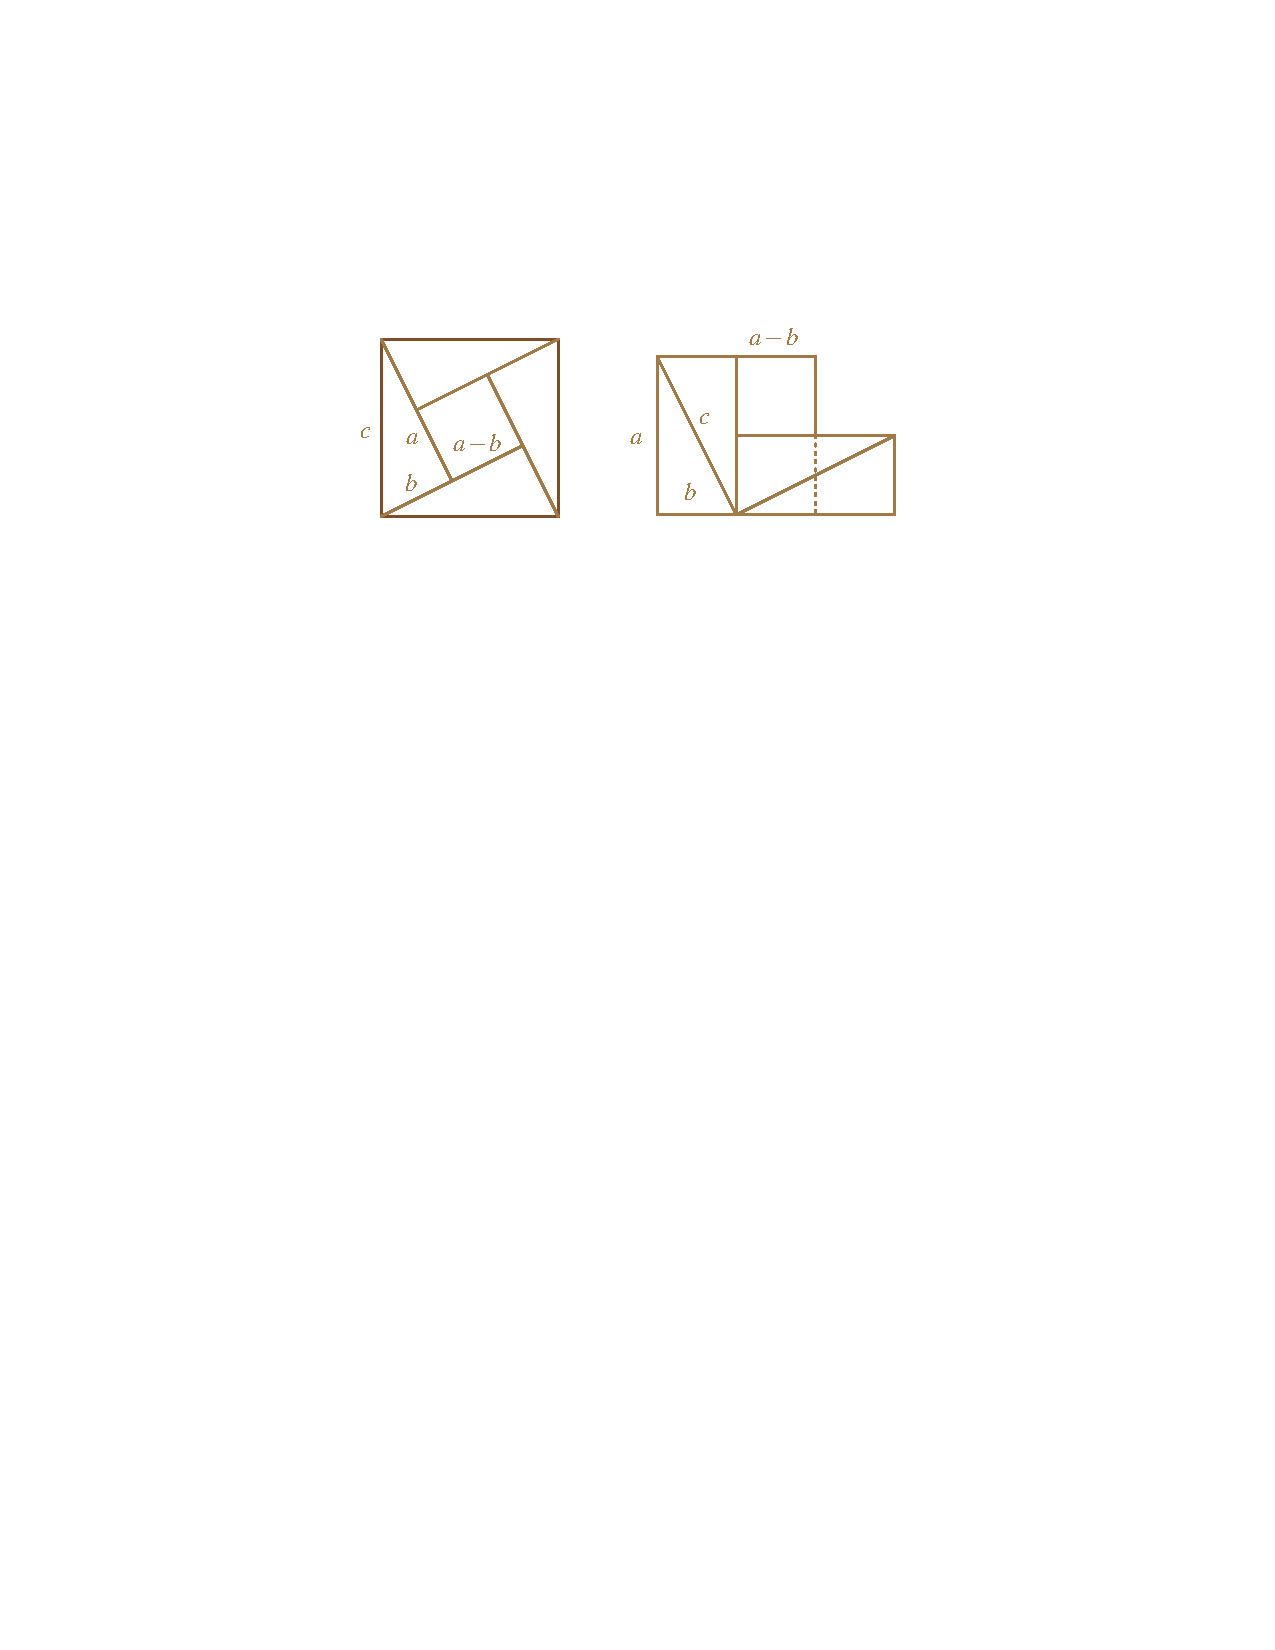
\includegraphics[width= 1\linewidth]{15}
		\caption{\small\textit{\color{lichsutoanhoc}Hình $3$. Chứng minh Định lý Pythagoras của Bhaskara.}}
		\vspace*{-10pt}
	\end{figure}
	Bạn đọc có thể tìm thêm các chứng minh định lý Pythagoras nhờ ghép hình và khoảng $400$ chứng minh khác trong các Tài liệu, thí dụ, [$5$].
	\vskip 0.1cm
	\textbf{\color{lichsutoanhoc}Phương trình  Pythagoras} 
	\vskip 0.1cm
	Định lý Pythagoras thể hiện mối quan hệ giữa định tính (tam giác vuông) và định lượng (đẳng thức liên hệ giữa độ dài các cạnh), một cách tự nhiên dẫn đến một bài toán số học tương ứng, được gọi là \textit{bài toán Pythagoras}. Bài toán này, một trong những bài toán sớm nhất trong lý thuyết số, yêu cầu tìm tất cả các tam giác vuông có các cạnh có độ dài nguyên, nghĩa là, tìm tất cả các nghiệm nguyên dương của \textit{phương trình Pythagoras}
	\begin{align*}
		{x^2} + {y^2} = {z^2}. \tag{$3$}
	\end{align*}
	Bộ ba $(x,y,z)$  các số nguyên dương thỏa mãn phương trình này được gọi là \textit{bộ ba Pythagoras}.
	\vskip 0.1cm
	Các tư liệu cổ viết rằng bản thân Pythagoras đã tìm ra các nghiệm dạng
	\begin{align*}
		\begin{array}{l}
			x = 2n + 1, y = 2{n^2} + 2n, \\
			z = 2{n^2} + 2n + 1,
		\end{array}\tag{$4$}
	\end{align*}
	trong đó $n \ge 1$  là một số nguyên tùy ý.
	\vskip 0.1cm
	Pythagoras có lẽ đã đi đến lời giải của mình bằng cách viết bình phương của một số qua bình phương nhỏ hơn ngay sau nó, cụ thể là
	\begin{align*}
		{k^2} = {(k - 1)^2} + (2k - 1). \tag{$5$}
	\end{align*}
	Bây giờ viết $2k-1$ dưới dạng bình phương của một số: $2k - 1 = {m^2}$.  Điều này có thể làm được, thí dụ, khi $k=5$  thì $2k-1= 9= 3^2$. Từ đây ta có $k = \frac{{{m^2} + 1}}{2}$  và   $k - 1 = \frac{{{m^2} - 1}}{2}$.
	\vskip 0.1cm
	Thay các giá trị này vào ($3$) ta được
	\begin{align*}
		{\left( {\frac{{{m^2} + 1}}{2}} \right)^2} = {m^2} + {\left( {\frac{{{m^2} - 1}}{2}} \right)^2}.
	\end{align*}
	Do đó
	\begin{align*}
		x = m,\quad y = \frac{{{m^2} - 1}}{2},\quad z = \frac{{{m^2} + 1}}{2} \tag{$6$}
	\end{align*}
	thỏa mãn phương trình Pythagoras với mọi $m>1$ lẻ ($m$  lẻ vì $m^2 = 2k-1$  là số lẻ). Đặt $m = 2n +1$  với $n \ge 1$  thì ($6$) có dạng ($4$).
	\vskip 0.1cm
	Thay  $n = 1,2,3,4,5$ ta được $5$ bộ ba đầu tiên:
	\begin{table}[H]
		\vspace*{-5pt}
		\centering
		\renewcommand{\arraystretch}{1.1}
		\begin{tabular}{|c|c|c|c|}
			\hline
			$n$ & $x$ & $y$ & $z$ \\
			\hline
			$1$	&$3$&	$4$&	$5$\\
			\hline
			$2$&	$5$&	$12$&	$13$\\
			\hline
			$3$&	$7$&	$24$&	$25$\\	
			\hline
			$4$&	$9$&	$40$&	$41$\\
			\hline
			$5$&	$11$&	$60$&	$61$\\
			\hline
		\end{tabular}
	\end{table}	
	Ta thấy, Pythagoras đã nhận được các bộ ba Pythagoras đặc biệt, với cạnh huyền lớn hơn cạnh góc vuông lớn một đơn vị.
	\vskip 0.1cm
	Bằng cách hai lần áp dụng ($5$), ta được
	\begin{align*}
		{\left( {k + 1} \right)^2} &= {k^2} + (2k + 1)\\
		&= \left( {{{\left( {k \!-\! 1} \right)}^2} \!+\! \left( {2k \!-\! 1} \right)} \right) \!+\! (2k \!+\! 1) \\
		&= {\left( {k - 1} \right)^2} + 4k.
	\end{align*}
	Đặt $k = n^2$.  Khi ấy  $4k = 4{n^2} = {\left( {2n} \right)^2}$.
	\vskip 0.05cm
	Phương trình Pythagoras trở thành
	\begin{align*}
		{\left( {{n^2} + 1} \right)^2} = {\left( {{n^2} - 1} \right)^2} + {\left( {2n} \right)^2}.
	\end{align*}
	Nhà triết học Hy Lạp Plato ($427-347$ trước Công nguyên) đã tìm được các bộ ba Pythagoras đặc biệt thỏa mãn phương trình Pythagoras, với cạnh huyền lớn hơn cạnh góc vuông lớn hai đơn vị
	\begin{align*}
		x = 2n,\,\, y = {n^2} - 1,\,\, z = {n^2} + 1. \tag{$7$}
	\end{align*}
	Nhận xét rằng bộ ba $(8, 15, 17)$ là bộ ba nhận được từ ($7$) mà không nhận được từ ($4$).
	\vskip 0.1cm 
	Cả hai công thức ($4$) và ($7$) hợp lại vẫn chưa vét hết nghiệm của ($3$). Euclid (thế kỷ III trước Công nguyên) trong quyển X của bộ \textit{Elements} (Cơ sở) đã đưa ra công thức nghiệm tổng quát của ($3$) là
	\begin{align*}
		x = 2mn,\,\, y = {m^2} - {n^2}, \,\, z = {m^2} + {n^2}, \tag{$8$}
	\end{align*}
	trong đó $m$  và $n$  là các số nguyên dương với $m >n$.
	\vskip 0.1cm 
	Diophantus (thế kỷ III) cũng đã đi đến công thức ($8$), có lẽ là như sau:
	\vskip 0.1cm
	Đặt $y = kx -z$, với $k$ là số hữu tỷ. Khi ấy
	\begin{align*}
		{z^2} - {x^2} = {y^2} = {\left( {kx - z} \right)^2} = {k^2}{x^2} - 2kxz + {z^2}.
	\end{align*}
	Dẫn tới $ - {x^2} = {k^2}{x^2} - 2kxz \Leftrightarrow x = 2kz - {k^2}x$.
	\vskip 0.1cm   
	Giải phương trình này theo $x$  ta được
	\begin{align*}
		x = \frac{{2kz}}{{1 + {k^2}}}.
	\end{align*}
	Suy ra 
	\begin{align*}
		y = kx - z = k\frac{{2kz}}{{{k^2} + 1}} - z = \frac{{{k^2} - 1}}{{{k^2} + 1}}z.
	\end{align*}
	Chọn $k = \frac{m}{n}$  với $m,n$  nguyên dương, $m >n$  ta được   $x = \frac{{2mn}}{{{m^2} + {n^2}}}z,\quad y = \frac{{{m^2} - {n^2}}}{{{m^2} + {n^2}}}z$.
	\vskip 0.1cm
	Đặt  $z = {m^2} + {n^2}$, ta có ($8$).
	\vskip 0.1cm
	Bài toán ngược là bất kỳ bộ ba Pythagoras nào cũng phải có dạng ($8$) chỉ được giải quyết triệt để vào thế kỷ X bởi các nhà toán học Ả Rập.
	\begin{figure}[H]
		\vspace*{-5pt}
		\centering
		\captionsetup{labelformat= empty, justification=centering}
		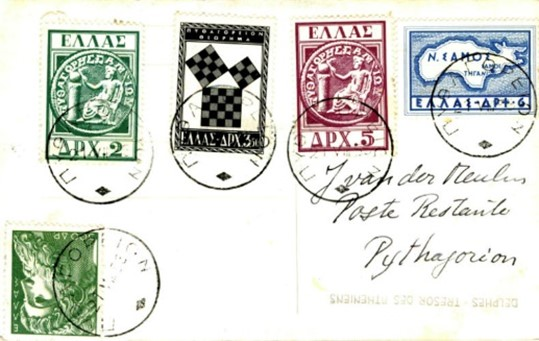
\includegraphics[width= 1\linewidth]{16}
		\caption{\small\textit{\color{lichsutoanhoc}Hình $4$: Một số tem thư vinh danh  Pythagoras.}}
		\vspace*{-10pt}
	\end{figure}
	\textbf{\color{lichsutoanhoc}Đại số hình học} (geometrical algebra) \textbf{\color{lichsutoanhoc}của trường phái Pythagoras}
	\vskip 0.1cm
	Có lẽ không phải chính Pythagoras, nhưng trường phái Pythagoras đã khởi đầu cho phương pháp \textit{đại số hình học} giải các bài toán dựng hình: dùng các chữ cái để biểu thị các đại lượng mô tả bởi các đối tượng hình học (độ dài, diện tích), từ đó đưa các bài toán dựng hình về giải các phương trình không quá bậc hai. Phương pháp \textit{đại số hình học} sau này đã được đưa vào bộ sách Cơ sở của Euclid [$2$]. Thí dụ, Mệnh đề II. $11$ trong [$2$]: ``Chia một đoạn thẳng thành hai phần sao cho diện tích hình chữ nhật có các cạnh là đoạn thẳng đó và một trong hai phần của nó bằng diện tích hình vuông có cạnh là đoạn còn lại" dẫn tới việc giải phương trình bậc hai 
	\begin{align*}
		a\left( {a - x} \right) = {x^2} \Leftrightarrow {x^2} + ax - {a^2} = 0.
	\end{align*}
	Nhiều bài toán sử dụng phương pháp đại số hình học có thể được xem thêm trong [$2$].
	\vskip 0.1cm
	\textbf{\color{lichsutoanhoc}Số vô tỷ}
	\vskip 0.1cm  Từ Định lý Pythagoras, ta dễ dàng suy ra rằng đường chéo (bằng  $b = a\sqrt{2}$)  của hình vuông cạnh $a$  không thông ước với cạnh của nó, tức là không có một đoạn độ dài $m$  nào để $a= qm$  và $b = a\sqrt{2}= pm$ trong đó  $p$  và $q$ là hai số tự nhiên. Nói riêng, $\sqrt{2}$  không thể là số hữu tỷ, tức là không thể có hai số tự nhiên $p$  và $q$  sao cho $\sqrt{2} = \frac{p}{q}$.   Ngày nay, học sinh lớp $9$ có thể chứng minh điều này một cách dễ dàng. Thật vậy, ta có thể coi  $\frac{p}{q}$  là  phân số tối giản, tức là $p$  và $q$  có ước chung lớn nhất bằng $1$. Ta có
	\begin{align*}
		\sqrt 2  = \frac{p}{q} \Leftrightarrow 2 = \frac{{{p^2}}}{{{q^2}}} \Leftrightarrow {p^2} = 2{q^2}.
	\end{align*}
	Suy ra $p^2$  và do đó $p$   là số chẵn, $p = 2k$.  Vậy
	\begin{align*}
		2{q^2} = {p^2} = {\left( {2k} \right)^2} = 4{k^2} \Rightarrow {q^2} = 2{k^2}.
	\end{align*}
	Suy ra $q^2$  và do đó $q$   là số chẵn. Vô lý.
	\vskip 0.1cm
	Điều vô lý này dẫn đến sự xuất hiện một loại số mới, chưa hề có trước Pythagoras, là \textit{số vô tỷ}. Người ta đồn đoán rằng, do sự phát hiện này trái với học thuyết Pythagoras về số và quan hệ của số với vũ trụ, trường phái Pythagoras đã giữ kín bí mật này trong nhiều năm.
	\vskip 0.1cm
	Phát hiện ra một loại số mới, số vô tỷ, là một cuộc cách mạng thật sự trong toán học. 
	\begin{figure}[H]
		\vspace*{-5pt}
		\centering
		\captionsetup{labelformat= empty, justification=centering}
		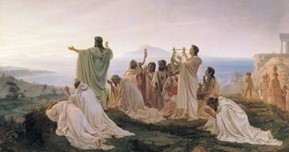
\includegraphics[width= 1\linewidth]{17}
		\caption{\small\textit{\color{lichsutoanhoc}Người Pythagoras đón mặt trời, 
				tranh: Fyodor Bronnikov $(1827-1902)$.}}
		\vspace*{-10pt}
	\end{figure}
	\textbf{\color{lichsutoanhoc}Kết luận}
	\vskip 0.1cm
	Những phương pháp chứng minh toán học của trường phái Pythagoras (kết hợp giữa số và hình, ...) không chỉ có ý nghĩa lịch sử, mà vẫn còn ý nghĩa thời sự trong dạy và học toán với định hướng phát hiện, khám phá và giải quyết vấn đề. Một bài báo không thể nói hết những gì mà Pythagoras và trường phái Pythagoras để lại cho nhân loại. Đã có khá nhiều sách viết về Pythagoras, bạn đọc có thể tìm được trên mạng. 
	\vskip 0.1cm 
	Ở Việt Nam, trong \textit{Ý Trai toán pháp nhất đắc lục}, Ý Trai Nguyễn Hữu Thận ($1757-1831$) là đã kết hợp định lý Pythagoras với phương pháp đại số hình học giải $60$ bài toán hình học. 
	\vskip 0.1cm
	\textbf{\color{lichsutoanhoc}Tài liệu tham khảo chính}
	\vskip 0.1cm
	[$1$] David M. Burton, \textit{The History of Mathematics}, An Introduction, Seventh Edition, McGraw--Hill, $2011$. Chapter $3$: \textit{The Beginnings of Greek Mathematics, $3.2$ Pythagorean Mathematics}, pp. $90-101$; $103-111$.
	\vskip 0.1cm
	[$2$] Euclid, \textit{Cơ sở của Hình học}, Nhà xuất bản Trí thức, $2016$, $350$ trang.
	\vskip 0.1cm
	[$3$] Thomas Heath, \textit{A History of Greek Mathematics}, Oxford at the Clarendon Press, $1921$, Volume $1$: \textit{From Thales to Euclid}, Chapter $3$: \textit{Pythagoras Arithmetic}, pp. $63-117$; Chapter $5$: \textit{Pythagorean Geometry}, pp. $139-169$.   
	\vskip 0.1cm
	[$4$] Victor J. Katz, \textit{A History of Mathematics, An Introduction}, Third Edition, Addison--Wesley, $2009$. Chapter $2$: \textit{The Beginnings of Mathematics in Greek}, $2.1.3$, \textit{Pythagoras and His School}, pp. $33-40$.
	\vskip 0.1cm
	[$5$] Eli Maor, \textit{The Pythagorean Theorem: A $4{,}000$ Year History}, Princeton University Press, $2007$, $259$ trang.
	\vskip 0.1cm
	[$6$] Nicomachus of Gerasa, \textit{Introduction to Arithmetic}, Translated into English by Martin Luther D’ooge, The Macmillan Company, New York, $1926$.
	\vskip 0.1cm
	[$7$]  \url{http://www.stichting-pythagoras.nl/}
	\vskip 0.1cm
	[$8$] Evans G. Valens, \textit{The Number of Things}, New York, E. P. Dutton \& Co. Inc., $1964$, $189$ trang.
\end{multicols}

